\capitolo{Pianificazione del Moto}
Pianificazione del moto significa scegliere la legge di moto, ossia \textit{La relazione matematica che esprime il moto in termini di posizione, velocità e accelerazione di un asse, motore o carico, in funzione di un parametro indipendente.}
\begin{itemize}
    \item Tempo, \(t [s]\)
    \item Posizione di un altro asse, \(q [m]\)
    \begin{itemize}
        \item Virtuale: camme elettroniche come clock di macchine
        \item Reale
        \begin{itemize}
            \item 2 assi meccanicamente accoppiati: camme meccaniche
            \item 2 assi accoppiati solo con controllo: camme elettriche
        \end{itemize}
    \end{itemize}
\end{itemize}

\paragrafo{Scelta delle Leggi di Moto}
Le specifiche in termini di legge di moto sono tendenzialmente poche, legate a: tempo di ciclo, spazio percorso, velocità minima, massima; a partire dalle quali va fatta una ottimizzazione consci di non poter ottenere una legge di moto perfetta.

\sottoparagrafo{Criteri di Scelta}
La scelta del tipo di legge di moto viene effettuata a partire da alcune caratteristiche progettuali:
\begin{enumerate}
    \item Minimizzazione di velocità massima o RMS
    \item Minimizzazione di accelerazione massima o RMS
    \item Minimizzazione dell'energia
    \item Minimizzazione della potenza
    \item Garantire realizzabilità della legge di moto in termini dinamici\footnote{In termini di banda passante di motore, controllo, di spettro della legge di moto e vibrazioni.}
\end{enumerate}
In generale la scelta dipende da progetto a progetto, tuttavia conviene cercare di avere focus su un parametro in particolare, perché diversi di questi risultano tra loro in trade off. Per esempio scegliere una forma d'onda di velocità triangolare senza riposi limita l'accelerazione massima al valore RMS, tuttavia questo potrebbe non permettere una buona scelta del motore per il quale non si andrebbe ad utilizzare la zona di lavoro intermittente.

\sezione{Formulazione delle principali leggi di Moto}
Le leggi di moto si dividono in due categorie: Punto-Punto (PP), quando le specifiche sono su punto di inizio e fine o Con specifiche su punti o tratti intermedi.
All'interno della tipologia Punto-Punto c'è un sottogruppo per cui la velocità inziale e finale sono nulle detto Rest-to-Rest (RtR).
In seguito verranno analizzati alcune leggi di moto del caso PP, con particolare attenzione ai sottocasi RtR.

Di particolare interesse è il moto simmetrico, ossia avente funzione velocità simmetrica rispetto \(\frac{T}{2}\).

\sottosezione{Parametrizzazione}
Per successive analisi conviene introdurre una normalizzazione dei tempi di accelerazione \(\lambda_A = \frac{t_A}{T}\) e decelerazione \(\lambda_D = \frac{t_D}{T}\), tenendo conto che per ciascuno vale \(0 < \lambda < 1\) e \(0 < \lambda_A + \lambda_D < 1\).

\paragrafo{Parametri di merito:}
A partire dalla parametrizzazione si possono ricavare per i vari parametri di progetto dei valori indipendenti da \(h\) alzata e \(T\) periodo di lavoro.
L'utilizzo di questi valori permette di semplificare la scelta della legge di modo fornendo delle figure di merito confrontabili, da porter tabellare.
\begin{itemize}
    \item \(C_V\) coefficiente di velocità massima
    \item \(C_{A+}\) coefficiente di accelerazione
    \item \(C_{A-}\) coefficiente di decelerazione
    \item \(C_A^{RMS}\) coefficiente di accelerazione RMS
\end{itemize}
Per poter ricavare dei valori generici è sufficiente ricavare la grandezza di cui interessa il coefficiente, considerando un alzata di 1 metro in un periodo di 1 secondo.

\sottosezione{Rampa di posizione}
Una rampa (limitata) di posizione è una legge di moto che descrive una funzione continua, ma non derivabile\footnote{Nel senso che la derivata destra e sinistra non coincidono in corrispondenza di punti di inizio e fine della rampa. Si considerano in seguito la velocità e l'accelerazioni come funzioni derivate da funzione definita a tratti.}; da questa legge di posizione si ottiene una velocità discontinua e accelerazione che tende all'infinito, cosa tuttavia irrealizzabile, perché richiederebbe motore a coppia infinita.

\sottosezione{Trapezoidale in velocità}
Una forma trapeziodale in velocità risulta in una funzione posizione continua e derivabile, di velocità continua ma non derivabile, quindi accelerazione discontinua, ma finita.
Nel caso di traiettoria RtR \( v_{fin} = 0 = \int^{t_{fin}}_{t_{in}} \acc{q} dt \), ossia le aree sottese dalla funzione accelerazione devono essere uguali.

\begin{figure}[h]
    \centering
    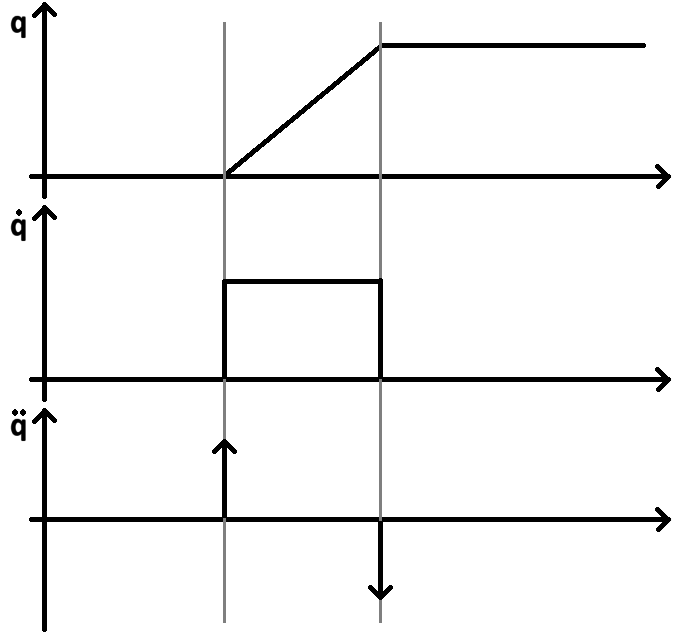
\includegraphics[width=0.3\textwidth]{Immagini/rampa_pos.png}
    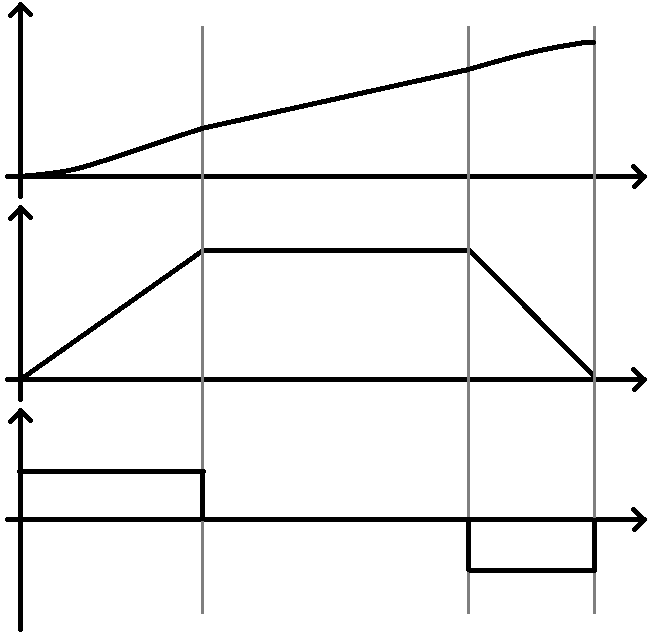
\includegraphics[width=0.3\textwidth]{Immagini/trapezoidale_vel.png}
    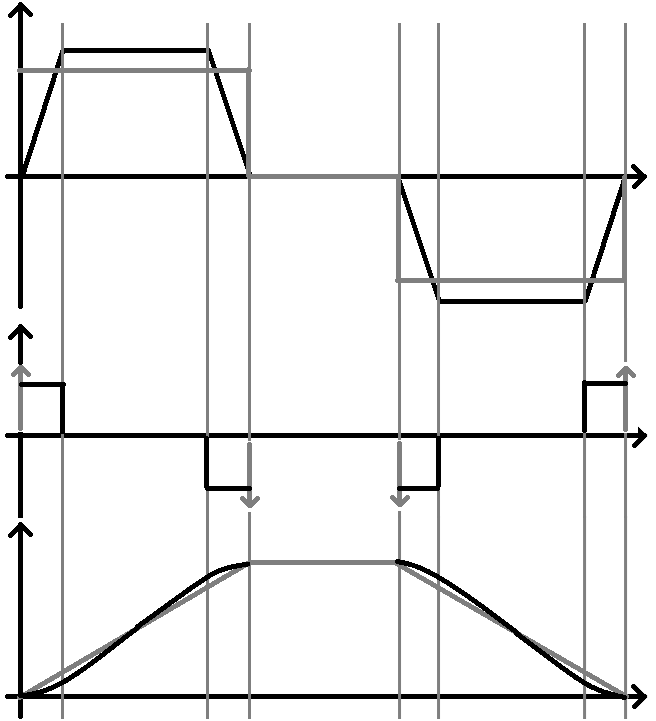
\includegraphics[width=0.3\textwidth]{Immagini/trapezoidale_acc.png}
    \caption{Rampa Posizione sx; Trapeziodale Velocità centro; Trapezoidale Accelerazione dx}
\end{figure}

\sottosottosezione{Grandezze significative (RtR)}
La velocità massima ottenibile si può determinare integrando la funzione di velocità, o più semplicemente facendo valutazioni geometriche sul trapezio, da cui si ottiene \(V_{max} = \frac{h}{\frac{t_A}{2}+t_C +\frac{t_D}{2}}\).
Possono essere ricavate di conseguenza l'accelerazione \(\abs{A} = \frac{V_{max}}{t_A}\) e la delecelazione \(\abs{D} = \frac{V_{max}}{t_D}\). Vale inoltre \(\frac{\abs{A}}{\abs{D}} = \frac{t_D}{t_A}\).

\paragrafo{Velocità con parametrizzazione:}
La velocità massima ottenibile diventa \(V_{max} = \frac{h}{T} \frac{1}{1-\frac{\lambda_A}{2}-\frac{\lambda_D}{2}}\), dove \(v_{media} = \frac{h}{T}\) ed è indipendente dalla traiettoria, viene definito \(C_v = \frac{1}{1-\frac{\lambda_A}{2}-\frac{\lambda_D}{2}}\).

\paragrafo{Accelerazione con parametrizzazione:}
L'accelerazione ottenuta diventa \(A=\frac{h}{T^2} \frac{1}{\lambda_A}\frac{1}{1-\frac{\left(\lambda_A + \lambda_D \right)}{2}}\), dove \(a = \frac{h}{T^2}\) rappresenta l'equivalente valore in caso di moto con accelerazione costante, da cui viene definito \(C_{A+} = \frac{1}{\lambda_A}\frac{1}{1-\frac{\left(\lambda_A + \lambda_D \right)}{2}}\).
In modo del tutto simile, associata alla decelerazione \(D\), viene definito \(C_{A-} = \frac{1}{\lambda_D}\frac{1}{1-\frac{\left(\lambda_A + \lambda_D \right)}{2}}\).

\paragrafo{Accelerazione RMS:}
L'accelerazione RMS si ottiene calcolando l'integrale usando le valutazioni geometriche per l'accelerazione e ricordando il legame tra \(\abs{D}\) e \(\abs{A}\), da cui si può ricavare l'espressione finale \(\acc{q}^{RMS} = \frac{h}{T^2} C_A \sqrt{\lambda_A + \frac{\lambda_A^2}{\lambda_D}}\), in cui viene definito \(C_A^{RMS} = C_A \sqrt{\lambda_A + \frac{\lambda_A^2}{\lambda_D}}\).
Analizzando la funzione si otttiene un minimo assoluto per \(\lambda_A=\lambda_D =\frac{1}{3}\), valori in corrispondenza dei quali si ottiene un moto simmetrico (equamente distribuito tra accelerazione, velocità costante e decelerazione).

\paragrafo{Potenza meccanica:}
Nel moto trapezoidale in velocità i punti più critici in termini di velocità sono per termine di fase di accelerazione e inizio fase di decelerazione, per cui si hanno \(\max{\acc{q}}\) e \(\max{\dot{q}}\), che portano ad avere, nel caso inerziale, \(\max{W_M}\) proporzionale a \(\max{\acc{q}} \cdot \max{\dot{q}}\).
A partire dalla potenza massima, si può definire il coefficiente di potenza massima come \(C_W = C_V C_A = \frac{1}{\lambda(1-\lambda)(1-\lambda)}\) nel caso di moto simmetrico.

\sottosottosezione{Legge trapezoidale con moto simmetrico, RtR}
Nel caso di legge trapezoidale con moto simmetrico, vale \(\lambda_A=\lambda_D := \lambda \in (0,1/2]\), i coefficienti diventano: \(C_V = \frac{1}{1-\lambda}\); \(C_A = \frac{1}{\lambda}\frac{1}{1-\lambda}\); \(C_A^{RMS} = C_A \sqrt{2\lambda}\).

\begin{figure}[h]
    \centering
    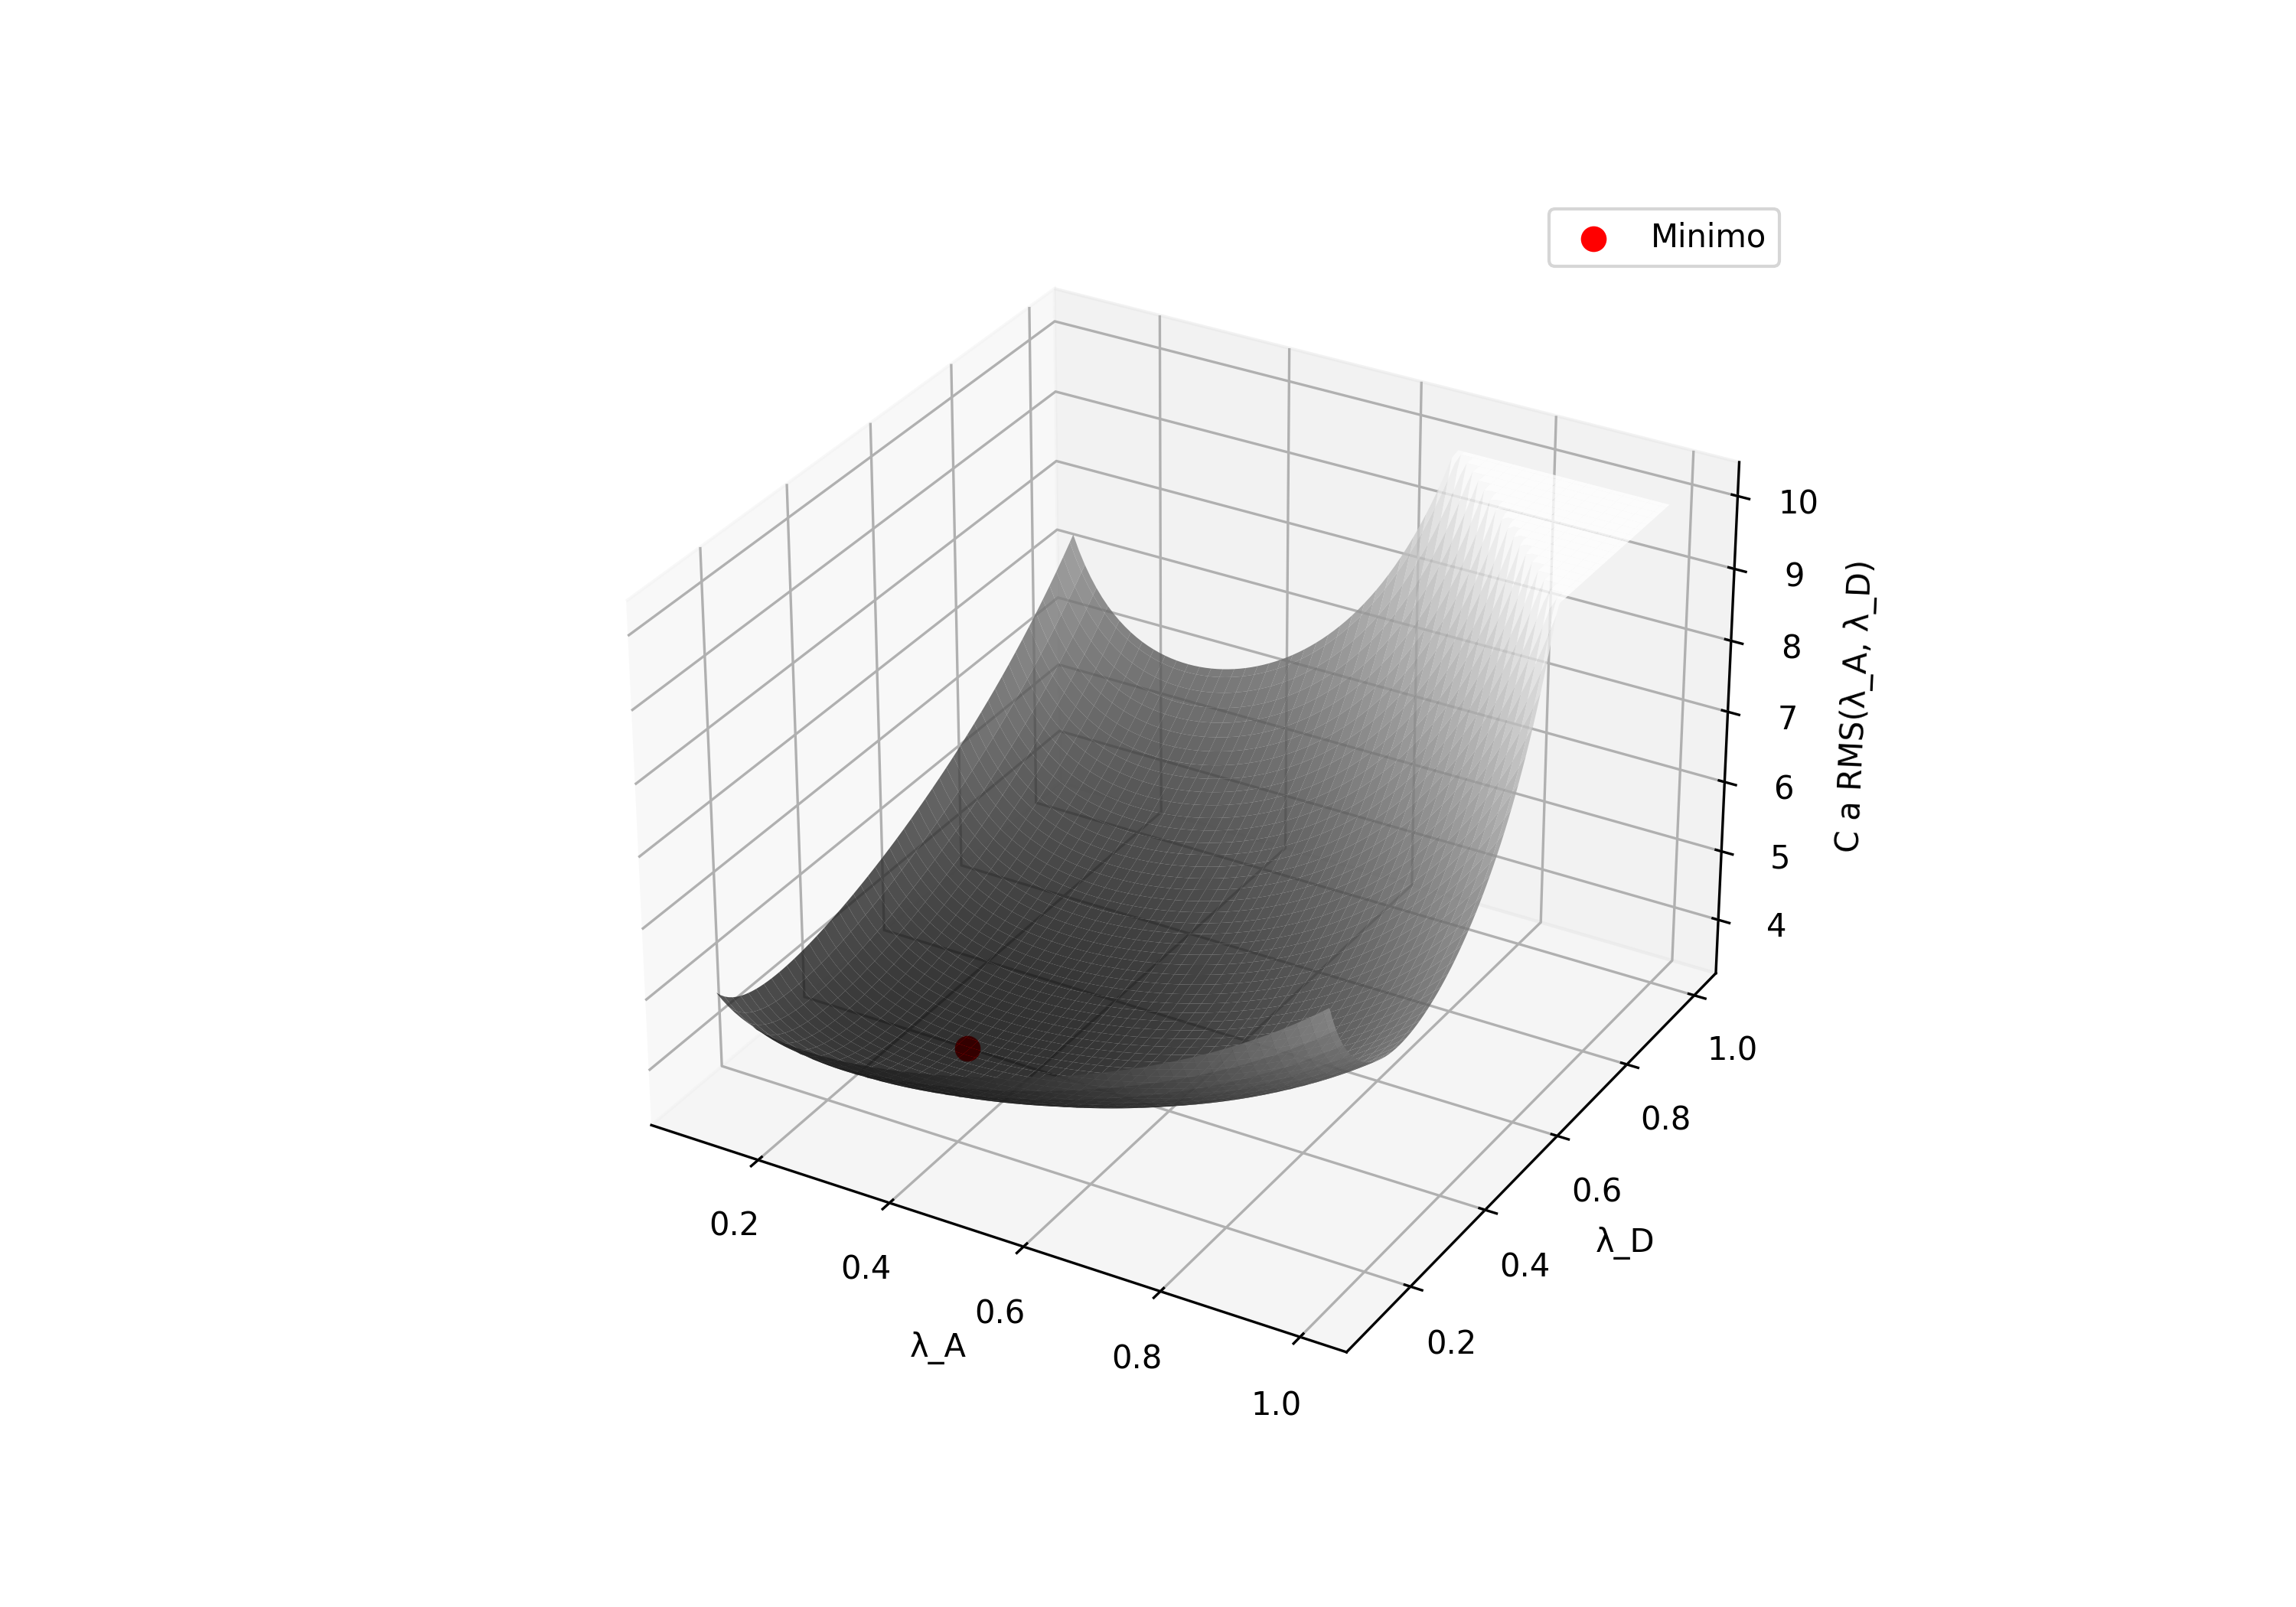
\includegraphics[width=0.4\textwidth]{Immagini/CaRMS.png}
    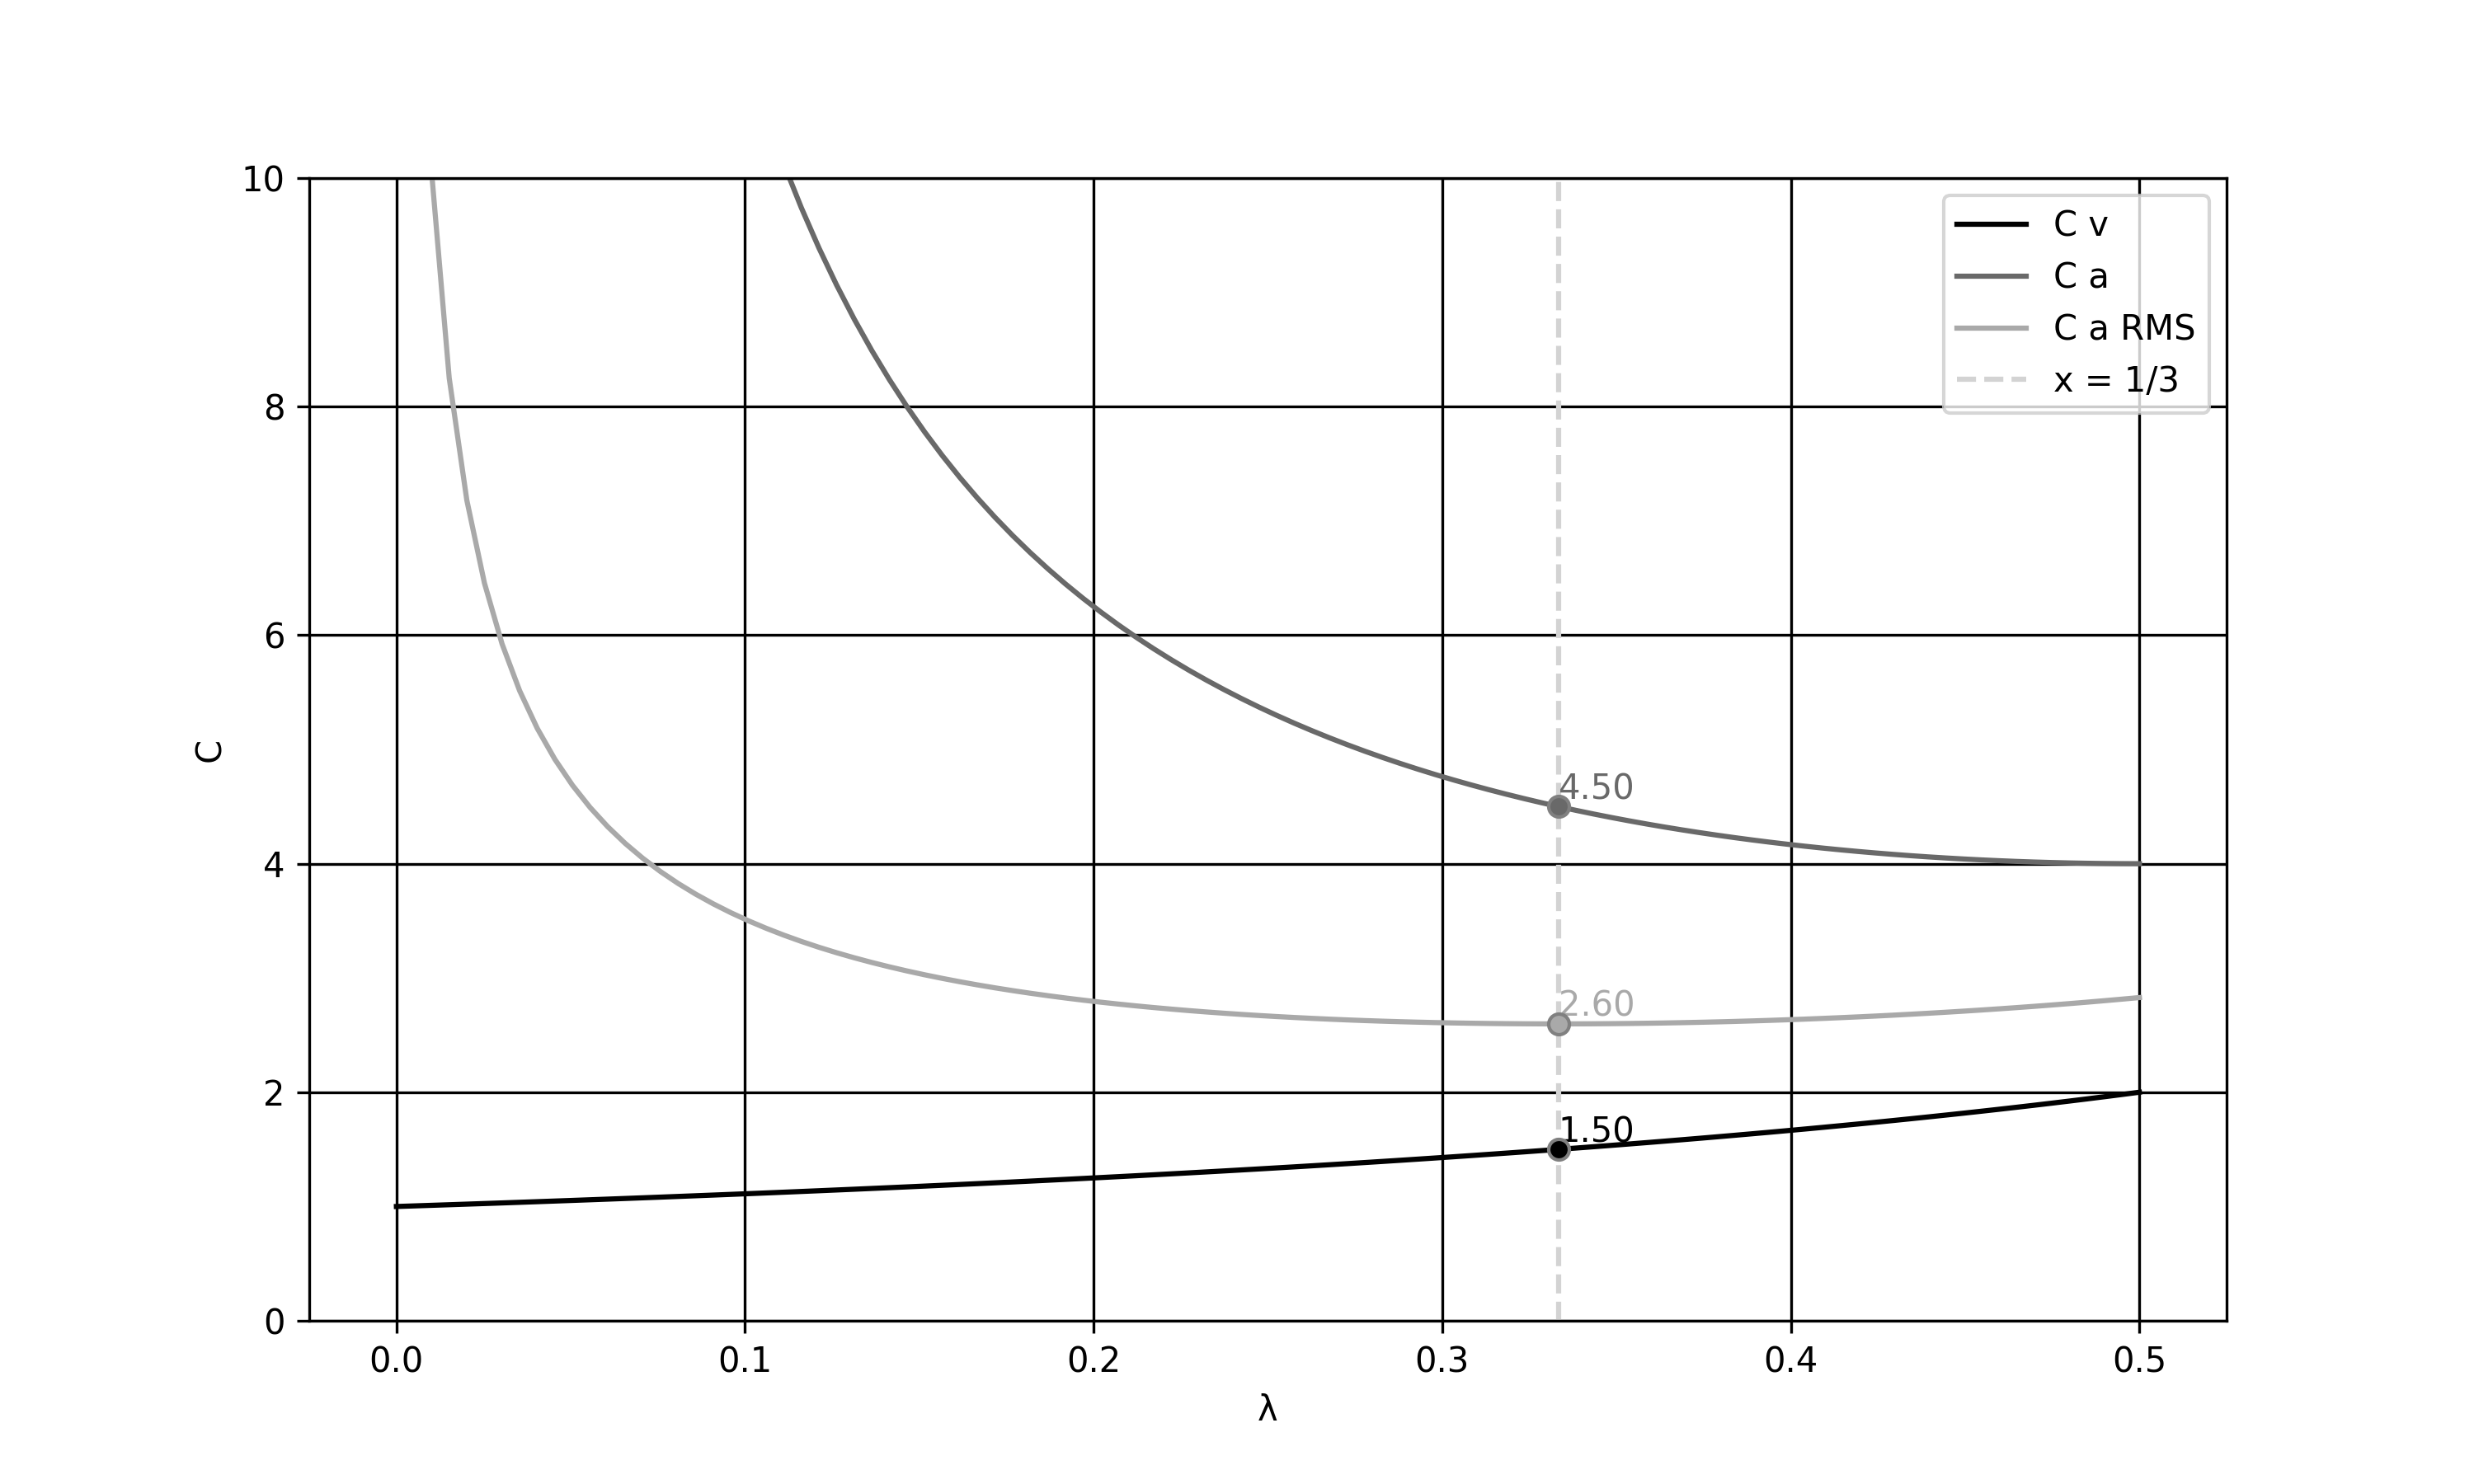
\includegraphics[width=0.55\textwidth]{Immagini/CvCaCaRMS.png}
    \caption{Coeff accelerazione RMS sx; Coeff per caso moto simmetrico dx}
\end{figure}

In questo caso risulta chiaro come ci sia un trade-off tra velocità e accelerazione.
Una prima scelta sensata (da cui partire per poi affinare la ricerca) potrebbe essere \(\lambda = \frac{1}{3}\), valore per cui si ha il minimo di coefficiente di accelerazione RMS, un basso coefficiente di accelerazione e un valore abbastanza basso di coefficiente di velocità, infine è anche prossimo all'ottimo energetico.

\paragrafo{Simmetria vs Assimetria:}
Quando c'è una disparità tra forze esterne in accelerazione e decelerazione (es ascensore o piano inclinato), conviene utilizzare una legge assimetrica al posto di una simmetrica per distribuire meglio le due aree.
In modo del tutto equivalente si può utilizzare l'espressione ottenuta per il caso simmetrico anche per il caso asimmetrico introducendo un \(\lambda_m=\frac{\lambda_A+\lambda_B}{2}\).

\sottosezione{Trapezoidale in Accelerazione}
A partire da una legge trapezoidale in velocità, considero di fare una legge trapezoidale in accelerazione che abbia la stessa velocità massima, questo influenza la scelta dei raccordi\footnote{Nel caso in figura i raccordi sono lineari, tuttavia potrebbero essere polinomiali, esponenziali, sinusoidali, ecc nel caso debbano essere modificati i coefficienti o migliorato lo spettro della legge di moto.}.
Infatti per ottenere la stessa velocità massima le aree delle due accelerazione deve essere uguale; a seguito di semplici valutazioni geometriche si può ricavare l'accelerazione massima per la trapezoidale in accelerazione come \(A_m=\frac{h}{T^2}\frac{1}{\lambda}(1-\lambda)(1-\gamma)\), dove \(\gamma = \frac{t_R}{t_A}\) ossia il tempo di raccordo normalizzato al tempo totale di accelerazione. 
In questa legge di moto l'accelerazione risulta continua, cosa che aumenta la semplicità realizzativa, vengono ridotte le vibrazioni, ma aumentano l'accelerazione massima e RMS.


\sottosottosezione{Jerk}
Il jerk è la derivata nel tempo dell'accelerazione. Un jerk finito porta ad avere accelerazione continua, si parla in questi casi di legge di moto dolci; un jerk infinito porta ad avere un'accelerazione discontinua, si parla quindi di leggi non dolci.
Anche per il jerk si può definire il coefficiente di jerk massimo \(\dddot{q} = \frac{h}{T^3}C_J\).
Nel caso di trapezoidale in accelerazione \(C_J = \frac{C_A}{\lambda \gamma}\)

\sottosezione{Polinomiale di Terzo Grado}
Si parla in generela di polinomiale per intendere una funzione polinomiale in posizione di un certo ordine.

Nel caso di terzo grado la legge di moto è definita dalle seguenti equazioni.
\[\begin{cases}
    q(t) = a_0 + a_1 (t-t_0) + a_2 (t-t_0)^2 + a_3 (t-t_0)^3 \\
    \dot{q}(t) = a_1 + 2 a_2 (t-t_0) + 3 a_3 (t-t_0)^2 \\
    \Ddot{q}(t) = 2 a_2 + 6 a_3 (t-t_0)
\end{cases}\]

Per definire univocamente il polinomio sono necessarie 4 condizioni, che solitamente sono:
\[\begin{cases}
    q(t_0) = q_{in}  \\
    q(t_0+T) = q_{fine}  \\
    \dot{q}(t_0) = \dot{q}_{in}  \\
    \dot{q}(t_0+T) = \dot{q}_{fine}  
\end{cases}\]
E a partire dalle quali è possibile ottenere i coefficienti \(a_0,a_1,a_2,a_3\).

Nel caso di polinomiale di terzo grado avente \(h=1, \ T=1, \ t_0=0\) le espressioni della legge di moto, per \(t\in[0,T]\), diventano:
\[\begin{cases}
    q(t) = 3 t^2 - 2 t^3 \\
    \dot{q}(t) = 6 t + 6 t^2 \\
    \Ddot{q}(t) = 6 - 12 t \\
    \dddot{q}(t) \neq -12 \ !!!
\end{cases}\]

Prestare estrema attenzione al calcolo del jerk, perchè per leggerezza si potrebbe scrivere \(\dddot{q}(t) = -12\), tuttavia sarebbe scorretto, perché nei punti di estremo la velocità non è nulla, ciò significa che le tangenti destra e sinistra sono diverse, per quei valori il jerk è infinito.

Per quanto riguarda i coefficienti tenere da conto che la polinomiale di terzo grado ha il valore minimo per quanto riguarda i coefficienti di accelerazione RMS di tutte le leggi di moto classiche. I valori sono: \(C_V=1.5, \ C_A = 6, \ C_A^{RMS}=3.4, \ C_J = \infty\)

\begin{figure}[h]
    \centering
    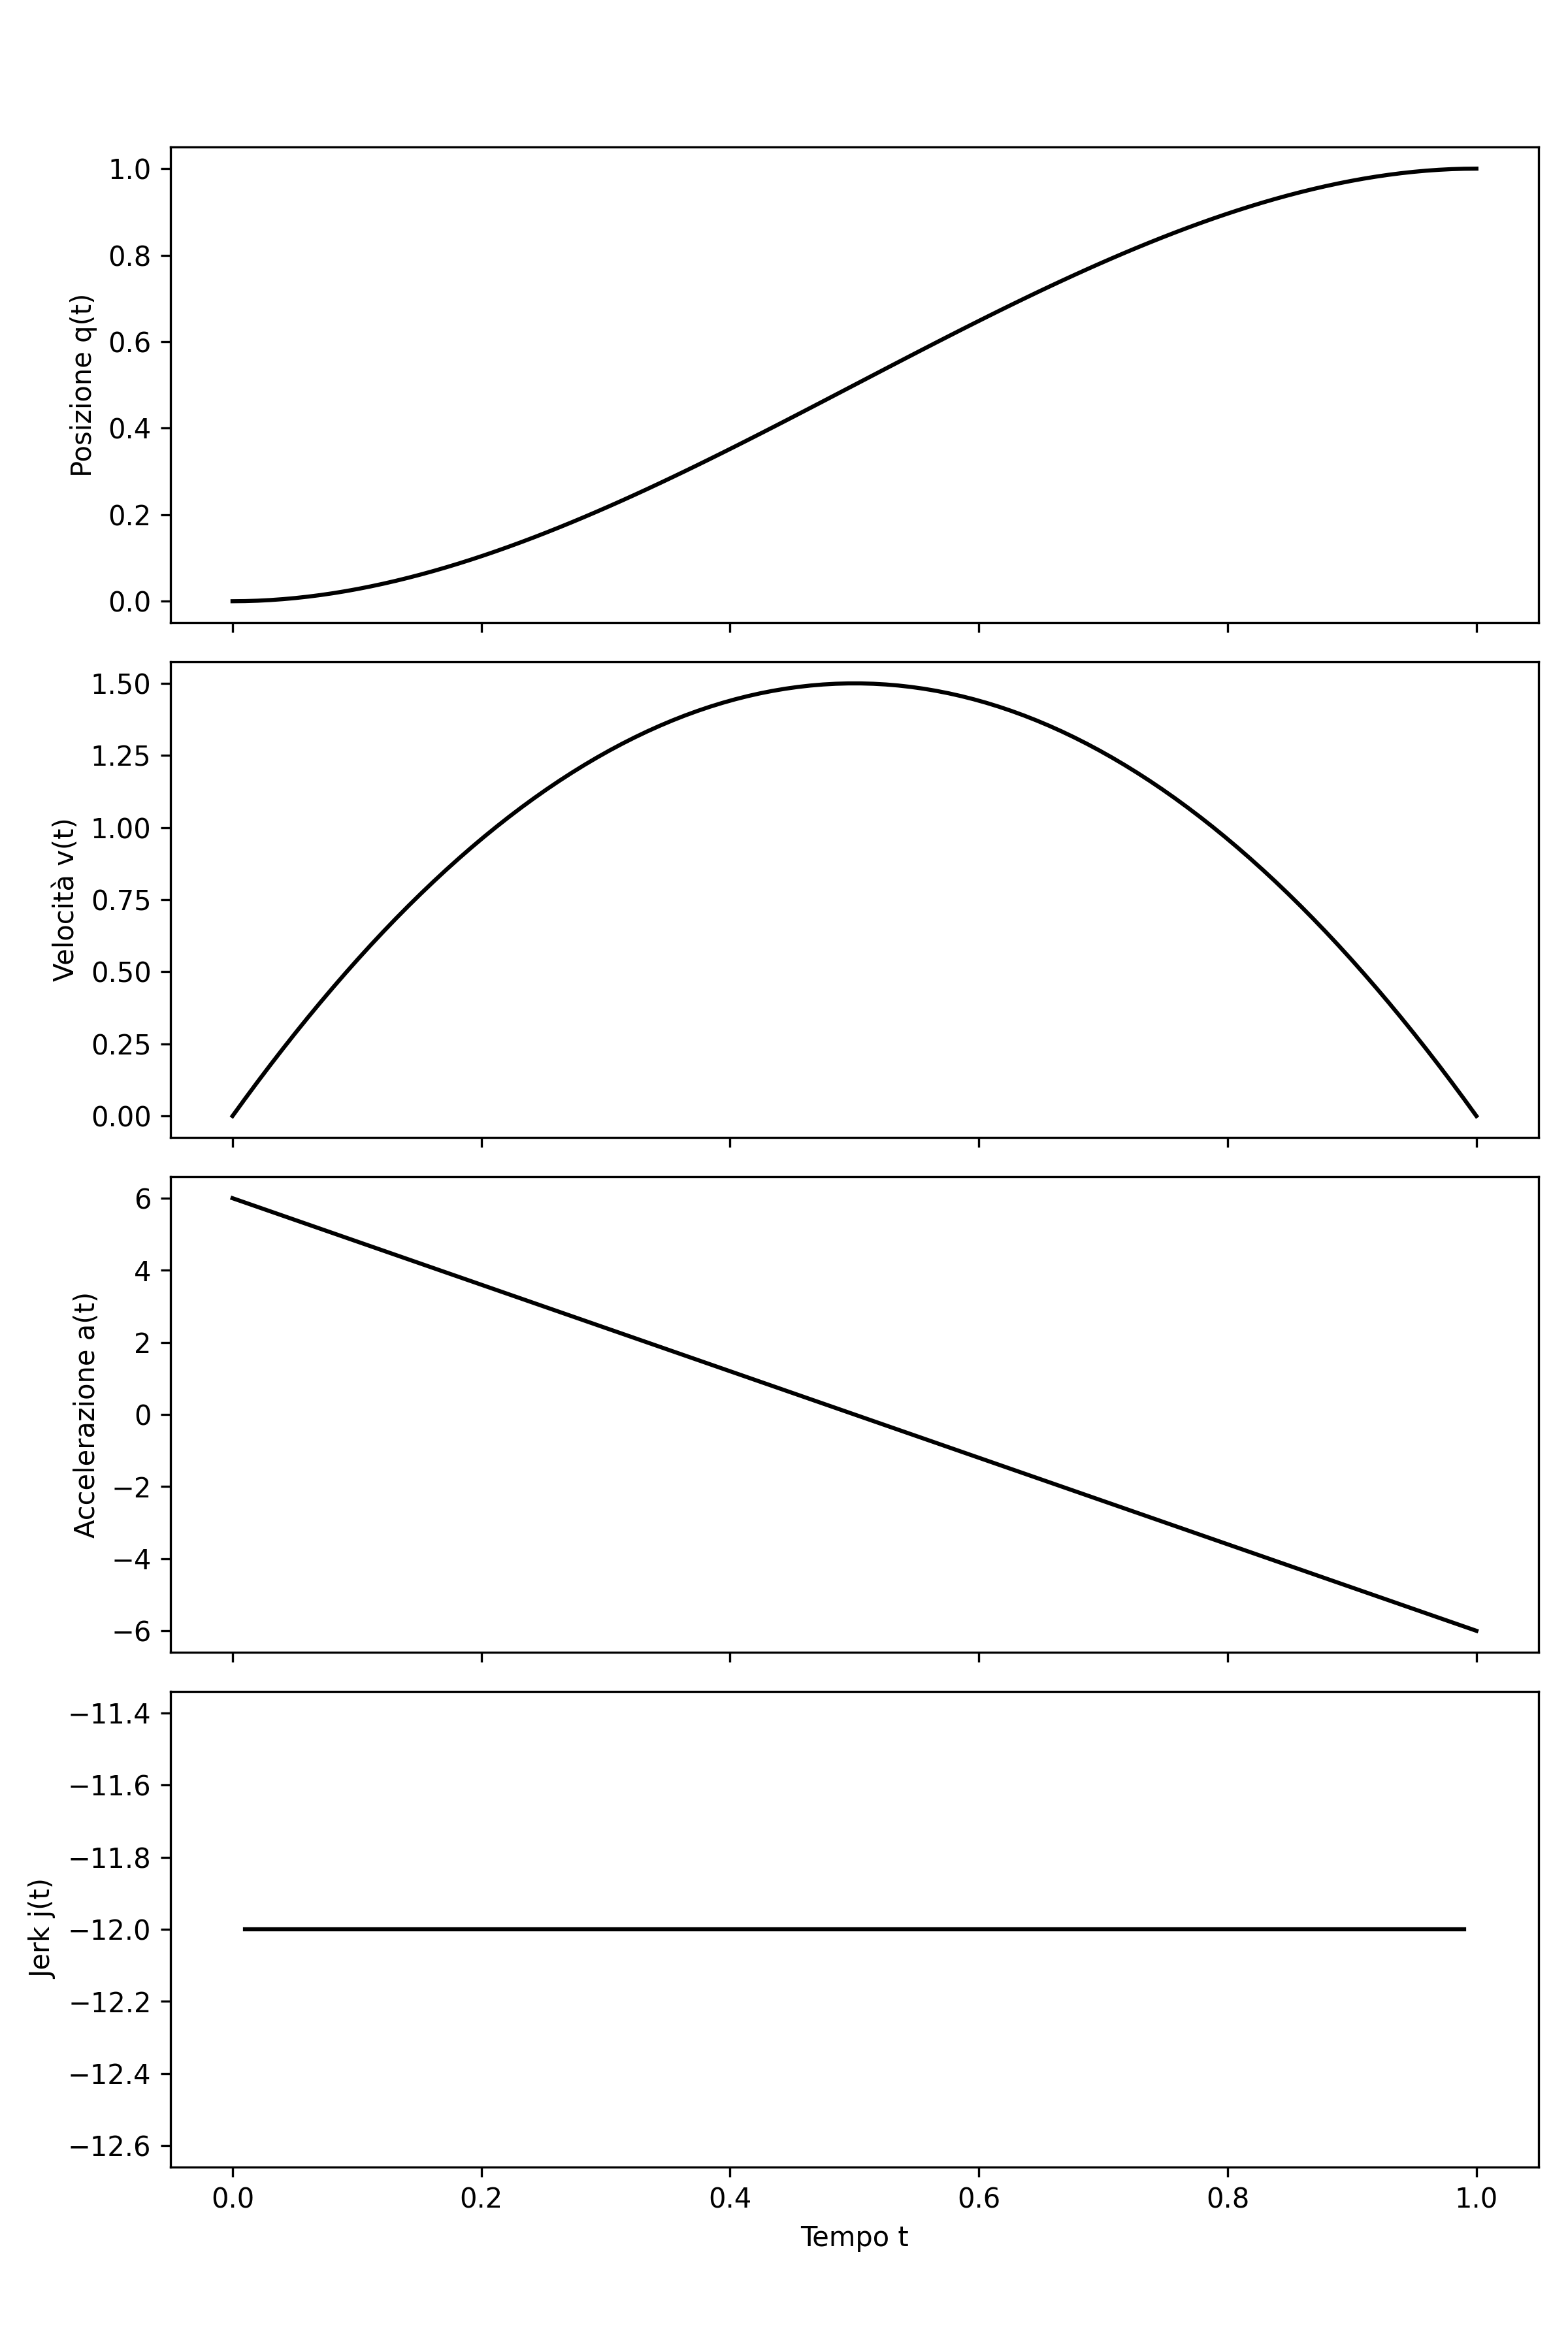
\includegraphics[width=0.3\textwidth]{Immagini/polinom_terzo_grado.png}
\end{figure}